%!TEX root = ../report.tex
\chapter{Methodology}

\section{Data}
Just like any other machine learning project the data is the most important part of the evaluation. Hence for the proper qualitative evaluation a deeper look at the data and how it was generated is needed.
The data set for training and testing are both obtained from Valdenegro et al \cite{stateoftheart}. Following is a brief description of the overall pipeline to obtain the data for training.

\subsection{Sonar image capture procedure}
In Valdenegro et al \cite{stateoftheart} the authors have explained in details how the raw sonar images were captured. In a water tank in their facility, the images were taken using ARIS Explorer 3000 and
mounted forward looking sonar(FLS). The objects featured are household garbage items and common marine debris. There are total 9 different types, such as metal cans, bottles, drink carton, metal chain, propeller, tire, hook, valve. 
In \cite{stateoftheart}, in controlled underwater environment total of 2072 images; about 2500 instances of the aforementioned objects were captured and labeled with 9 classes accordingly.

\subsection{Data generation for deep learning}
\begin{figure}[ht]
\centering
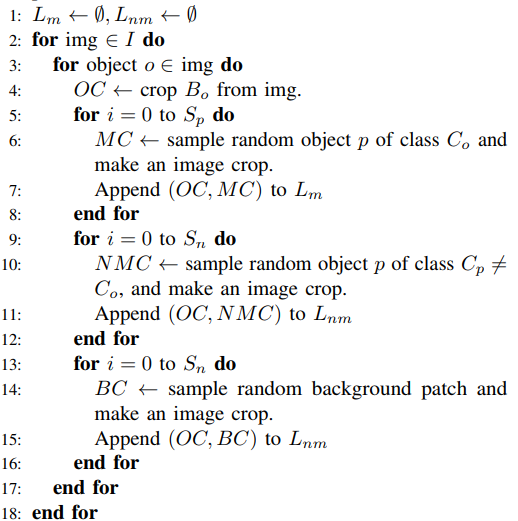
\includegraphics[height= 8cm]{images/densenet/training_data_generation}
\caption{Algorithm for matching and non matching pair of patch generation from Valdenegro et al \cite{stateoftheart}}
\label{fig:training_data_generation}
\end{figure}

As part of the same work \cite{stateoftheart}, matching and non-matching pairs 
of sonar image patches were generated using a patch generation algorithm displayed in figure \ref{fig:training_data_generation} where each patch, an instance of one of the 9 classes, were obtained from meaningful crops of the original 
sonar images. Authors have figured that 96x96 pixels is the best size of the crops.

\begin{figure}[ht]
\centering
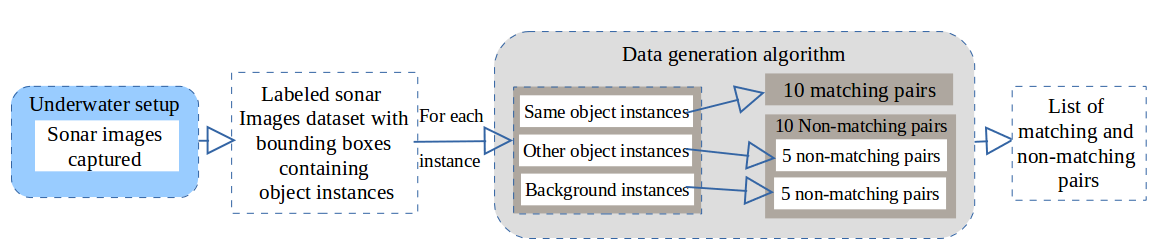
\includegraphics[width= 14cm]{images/densenet/data_pipeline2}
\caption{Data processing pipe line}
\label{fig:data_pipeline}
\end{figure}

To create matching pair, two patches that belong to the same object-type but different perspective and insonification level were used. For generating non-matching pair, two instances of different 
object-types were used. Also, one instance of an object and a background patch, which contains no object instance, were used to generate additional non-matching patches. According to the authors of \cite{stateoftheart}, 
for balanced and effective learning, the ratio of matching and non-matching pairs in both train and test data is maintained at 1:1. That is, for every ten matching pair five object-object non-matching 
and five object-background non-matching pairs were generated. In figure \ref{fig:data_pipeline} the overall pipeline for the data generation is displayed in simple block diagram.
In figure \ref{fig:generated_patches} some sample patches from all type of pairs are displayed. Using the patch generation algorithm total of 
39840 pairs were generated from the instances of 6 distinct object type, which were used as the train data.
While another 7440 pairs were generated from the instances of remaining object types, for testing purpose. This test dataset does not contain any common object with the training dataset,
it should be a good test for the generalization of the approaches. The labels for the data are 0 and 1 representing non-matching and matching pairs respectively. 
For this thesis work, this dataset is obtained in HDF5 files \cite{hdf5}. It contains patches in form of tensors \cite{tensors}, each of shape (2,96,96). Here the pair of patches (size 96x96) are placed in a way that each channel
contains one patch. %For final comparison of performance the same test data will be used.

\begin{figure}[ht]
\centering
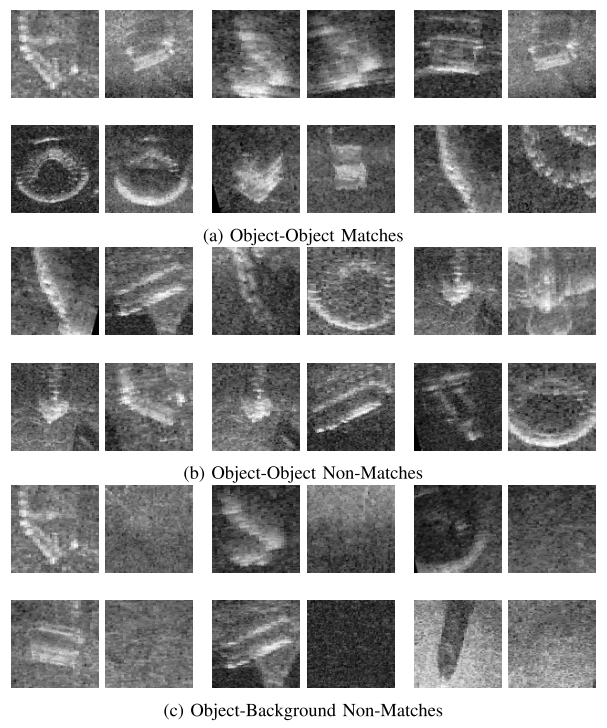
\includegraphics[height= 13cm]{images/densenet/generated_patches}
\caption{Some sample of the matching and non-matching pairs from Valdenegro et al \cite{stateoftheart}}
\label{fig:generated_patches}
\end{figure}

\flushbottom
\newpage
\section{Architectures}

\subsection{Densenet}
In Densenet each layer connects to every layer in a feed-forward fashion. 
With the basic idea to enhance the feature propagation, each layer of Densenet blocks takes the feature-maps of the previous stages as input.  
\begin{figure}[ht]
\centering
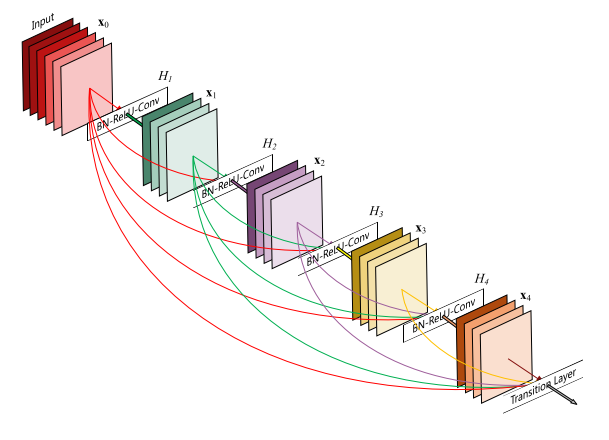
\includegraphics[width=0.5\textwidth]{images/densenet/densenet.png}
\caption{Densenet structure.}
\label{fig:densenet}
\end{figure}

\subsection{Contrastive loss}
Using contrastive loss higher dimensional input data (e.g. pair of images) can be mapped in the much lower dimensional output manifold, where similar pairs are placed closer to each other and 
the dissimilar pairs have bigger distances between them depending on their dissimilarity.  So using this loss function the “distance” between two input patches projected in the output manifold can be 
predicted and if the distance is closer to 0 then the input pairs are matching, otherwise its dissimilar (above threshold). The formula for the loss is shown below. 
\begin{figure}[ht]
\centering
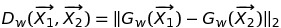
\includegraphics[height= 0.45cm]{images/contrastive/contrastive_loss_formula1.jpg}%TODO exchange this with the actual latex code
\label{fig:contrastive_loss_formula1}
\end{figure}

\begin{figure}[ht]
\centering
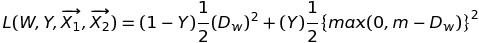
\includegraphics[height= 0.7cm]{images/contrastive/contrastive_loss_formula2.jpg}
\label{fig:contrastive_loss_formula2}
\end{figure}

Here L is the loss term, the formula presented here is the most generalized form of the loss function, suitable for batch training. 
$ \vec{X_1}$, $ \vec{X_2}$ represents a pair of input image vectors. Y are the labels, 0 for similar pair and 1 for dissimilar pair. $D_w$ is the parameterized distance function to be learned by the algorithm. 
m is the margin and m is always greater than zero and it defines a radius around $G_w$. The dissimilar pairs only contribute to the loss function if their distance is within the radius.
One of the idea for evaluating this loss function is to use it with a Siamese network, as the loss function takes a pair of images as input. So its very relevant to the problem statement of this thesis. 

The network structure is as follows, Conv(n, a x a)-Conv(n, a x a)-MP(2, 2)-Conv(2n, a x a)-Conv(2n, a x a)-MP(2, 2)-Conv(4n, a x a)-Conv(4n, a x a)-Conv(4n, a x a)-MP(2, 2)-Conv(8n, a x a)-Conv(8n, a x a)-Conv(8n, a x a)-MP(2, 2)-
Conv(8n, a x a)-Conv(8n, a x a)-Conv(8n, a x a)-MP(2, 2)-FC(d). It also evaluated if more FC(d) layers are needed for the network to perform well. If batch normalization improves the result, it is also evaluated. For evaluation batch norm
layer is added after the FC(d) layer. The a,n and d are the parameters which are obtained after doing grid search from a pre defined set of values. %TODO this needs polishing and moved to evaluation section

\section{Experimental Design}

\subsection{Search for best hyperparameters}
What are the hyperparameters.
Effect of setting best hyper parameters.

\begin{figure}[ht]
\centering
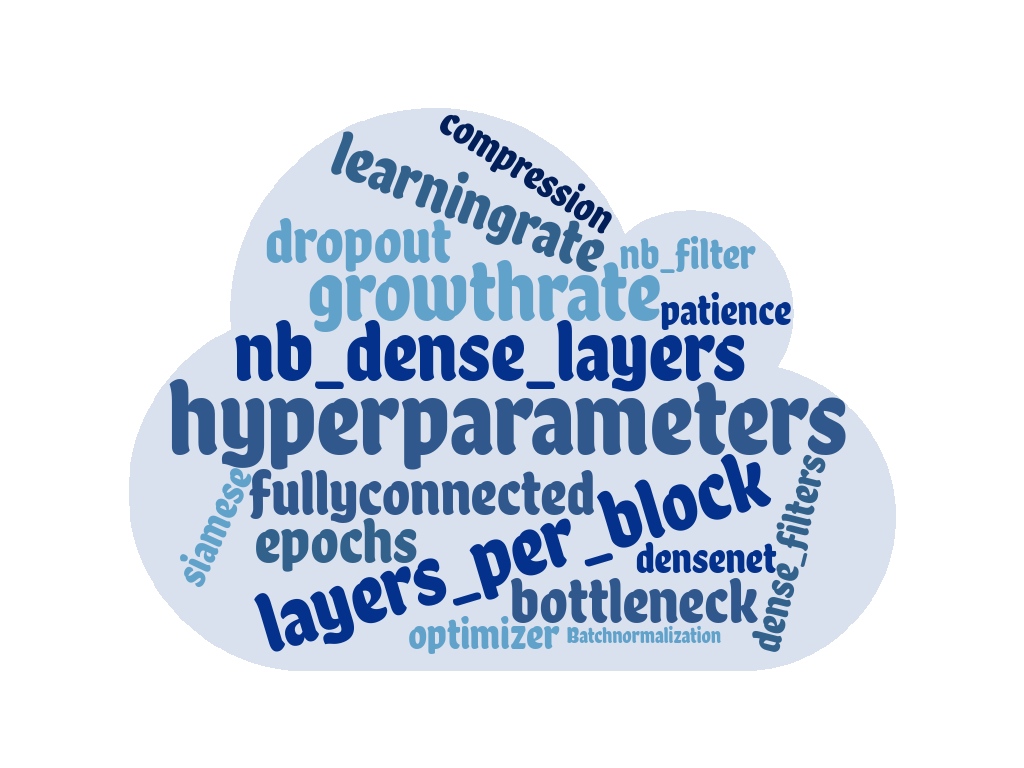
\includegraphics[width=0.5\textwidth]{images/densenet/wordcloud_hyperparameters.png}
\caption{\label{fig:wordcloud_hp}Hyper parameters word cloud.}
\end{figure}

\subsection{Grid search}
Currently the search space for the evaluation is hand designed and supplied to the evaluation script externally. Example
%\begin{figure}[ht]
%\centering
%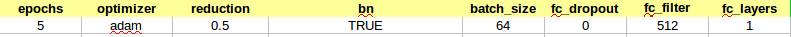
\includegraphics[width=1\textwidth]{images/densenet/test_cases.png}
%\caption{\label{fig:search_space}Custom grid search space example.}
%\end{figure}

\begin{table}
\centering
    \begin{tabular}{|c c c c c|} 
      \hline\hline
      Epochs & Optimizer & Batch size & Dropout & Use batch norm\\[0.5ex] 
      \hline
      5 & adam & 64 & 0.4 & True \\  
      \hline
      5 & adam & 64 & 0.4 & False \\ 
      %\hline
      %5 & adam & 64 & 0.7 & False \\ 
      %\hline
      %8 & rmsprop & 64 & 0.4 & True\\ 
      \hline \hline
    \end{tabular}
  \caption{Custom grid search space example.}
  \label{table:grid_example}
\end{table}

In this example it is displayed that how the search space is hand designed to evaluate different cases, here the effect of using batch normalization can be investigated by comparing the results of two test cases.
All the values set in the grid passed as input to the actual code and defines the structure or different parameters from inside  the code. In \ref{table:grid_example} the flag use batch norm is set to 'True', which
gets propagated in the actual block of code where it enables the use of batch normalization layer, where applicable. 

For the evaluation the epochs are set after multiple testings in order to ensure, to some extend, the networks does not get too overtrained and the generalization gets poorer. Also if the network is undertrained, then 
it will not generalize well. The setting the epochs were one of the big challenge of this work, because in some cases the networks gets overtrained after 4-5 epochs.

